\documentclass[a4paper]{article}
\usepackage[newfloat]{minted}
\usepackage{graphicx}
\usepackage{caption}
\usepackage{amsmath}
\usepackage{amsfonts}
\usepackage[a4paper,left=3cm,right=2cm,top=2.5cm,bottom=2.5cm]{geometry}
\usepackage[colorlinks=true, urlcolor=blue, pdfborder={0 0 0}]{hyperref}
\usepackage{subcaption}
\newenvironment{code}{\captionsetup{type=listing}}{}
\SetupFloatingEnvironment{listing}{name=Code}

\title{RL Homework 3}
\author{Ananth Mahadevan}
\begin{document}
\maketitle
\clearpage


\section*{Question 1}
The heatmap training times for $\epsilon=0.2$ and GLIE is seen in Figure~\ref{fig-training-cartpole}

\begin{figure}[h!]
    \centering
    \begin{subfigure}[b]{0.4\textwidth}
        \centering
        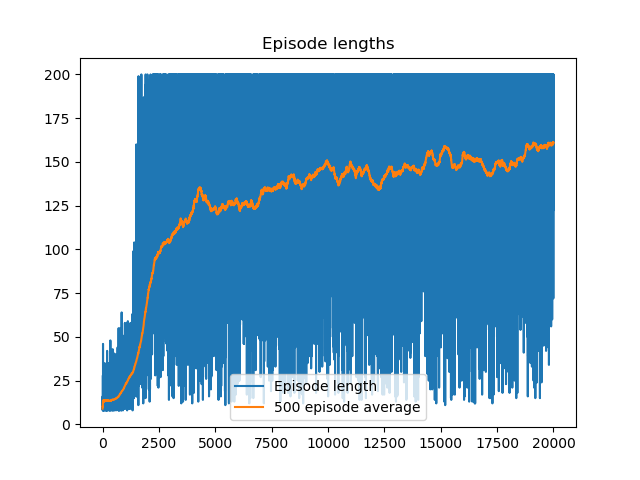
\includegraphics[width=\textwidth]{training_epsilon_0_2.png}
        \caption{$\epsilon=0.2$}
    \end{subfigure}
    \begin{subfigure}[b]{0.4\textwidth}
        \centering
        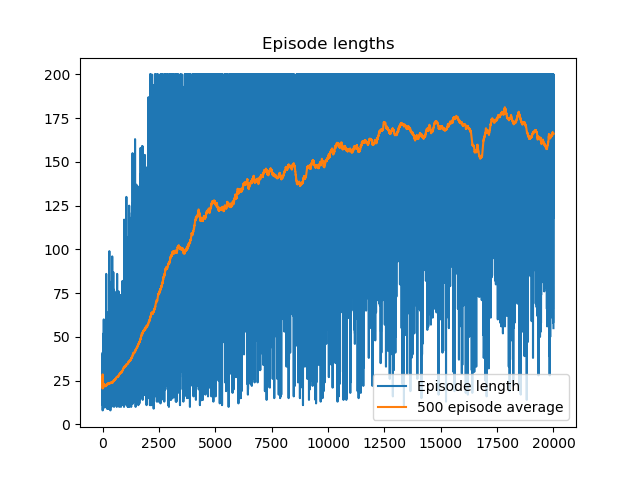
\includegraphics[width=\textwidth]{training_GLIE.png}
        \caption{GLIE}
        \label{fig-GLIE}
    \end{subfigure}
    \caption{Training Performance of constant $\epsilon$ and GLIE }
    \label{fig-training-cartpole}
\end{figure}

The heatmap for Task 2 is shown below
\begin{figure}[h!]
    \centering
    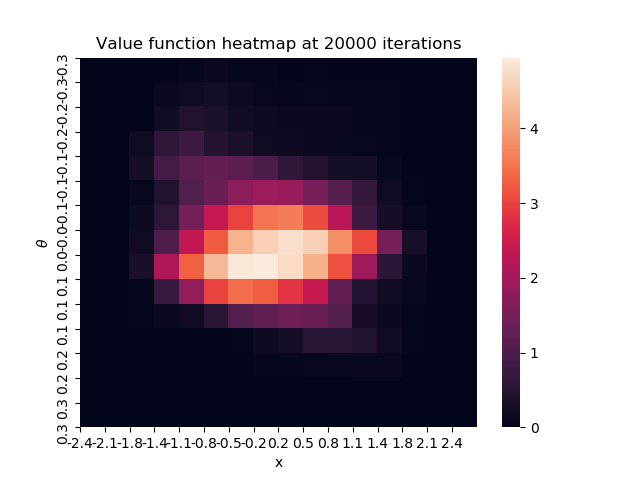
\includegraphics[width=\textwidth]{heatmap_done.png}
    \caption{Heatmap of value function}
    \label{fig-heatmap-done}
\end{figure}

\noindent
My hypothesis for what the heatmap of the value function would have looked like in the various cases are
\begin{itemize}
    \item \textbf{before training} \\ 
    Before training the heatmap would have be all uniformly zero as the value of the Q learning gird would be initialized to zero by before training and no value has been learnt yet.
    \item \textbf{after a single episode}\\
    After a single episode I guess it would update states very close to the center ($x=0$) and small angles. This change in the value will also be very small. This is because the first episode is most likely to fail and hence only the handful of states in which it managed to keep the pole upright would get a reward to have changed the Q learning grid's initial values of 0. And as the rewards would likely be low the change from 0 is also small.
    \item \textbf{Halfway through training}\\
    By this point I would expect the heatmap to more or less converge to roughly how the final heatmap would look. By this I mean that the exploration has been carried out until halfway through, would cover most of the states around the middle of the environment ($x=0$ and $\theta =0$). This is because it has explored most of the state space and as the value of $\epsilon$ is decreasing further the values will not change too much after the halfway point the amount of exploration will decrease and the values will just converge to a better level till the end of the episodes. This is also supported by the Figure~\ref{fig-GLIE} the average episode length is similar 
\end{itemize}
All of these claims can be verified by the plots of the heatmap as seen in 

\begin{figure}[h!]
    \centering
    \begin{subfigure}[b]{0.4\textwidth}
        \centering
        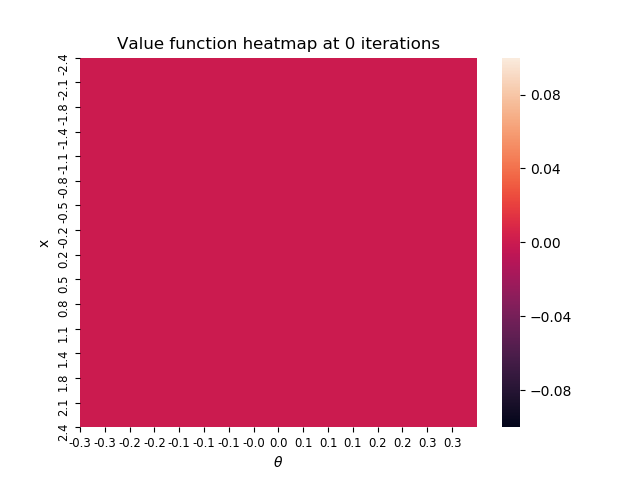
\includegraphics[width=\textwidth]{Heatmap_0.png}
        \caption{After 0 episodes}
    \end{subfigure}
    \centering
    \begin{subfigure}[b]{0.4\textwidth}
        \centering
        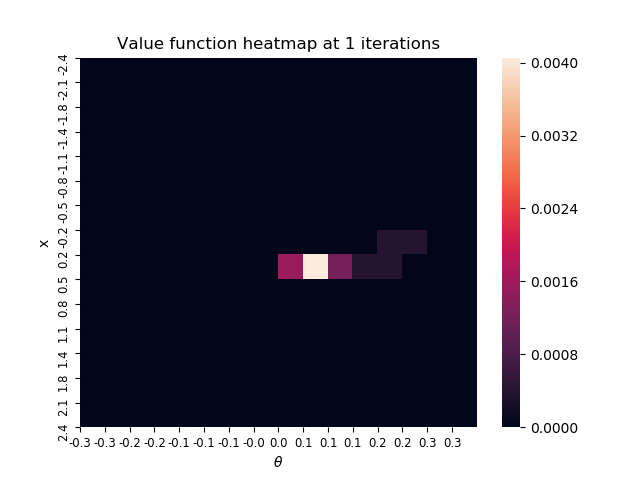
\includegraphics[width=\textwidth]{Heatmap_1.png}
        \caption{After 1 episodes}
    \end{subfigure}

    \begin{subfigure}[b]{0.5\textwidth}
        \centering
        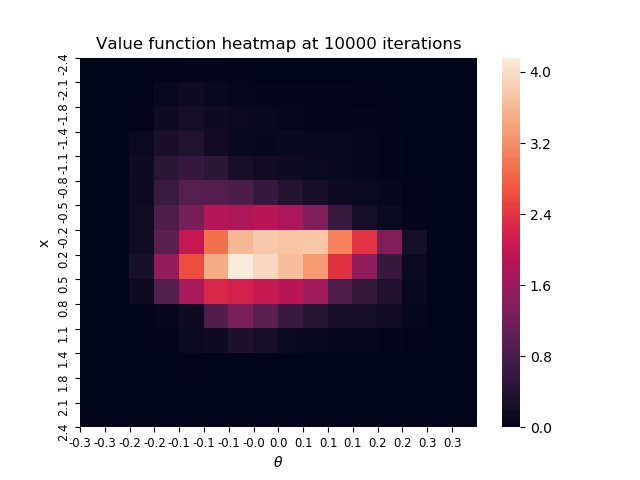
\includegraphics[width=\textwidth]{heatmap_10000.png}
        \caption{After 10,00 episodes (halfway)}
    \end{subfigure}
    \caption{Heatmap of Value function after different number of episodes}
    \label{fig-heatmap-diff}
\end{figure}

\section*{Question 2.1}
The training graphs for the two cases are seen Figure~\ref{fig-init-q}
\begin{figure}[h!]
    \centering
    \begin{subfigure}[b]{0.4\textwidth}
        \centering
        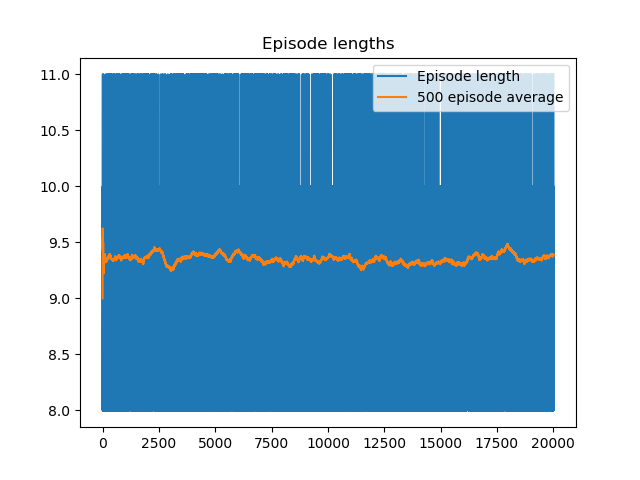
\includegraphics[width=\textwidth]{epsilon_0_init_0.png}
        \caption{Initial Q value = 0}        
    \end{subfigure}
    \begin{subfigure}[b]{0.4\textwidth}
        \centering
        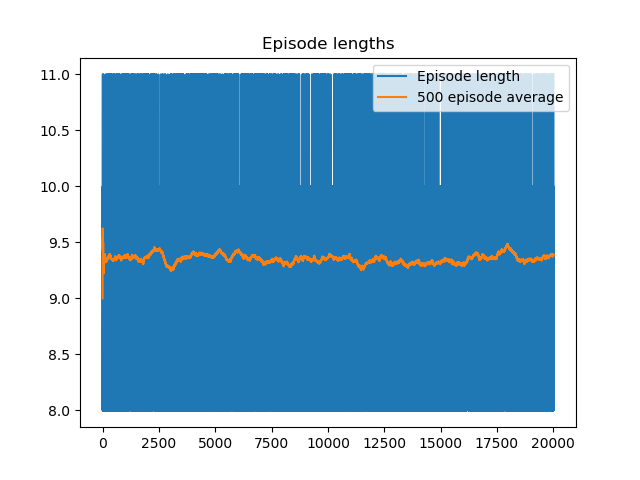
\includegraphics[width=\textwidth]{epsilon_0_init_50.png}
        \caption{Initial Q value = 50}        
    \end{subfigure}
    \caption{Training Performance of $\epsilon=0$ and different initial Q values}
    \label{fig-init-q}
\end{figure}

Based on these plots we can see that the case when $\texttt{q\_init}=50$, the model is able to stay alive longer and also has much better rewards than the model when \texttt{q\_init}=0. 
\section*{Question 2.2}
When the initial value of the Q learning grid is 0 and the $\epsilon$ is also $0$, this means that the policy will just choose to be greedy. But because the state space hasn't been explored at all the exploitation of the rewards is also the little it gets. In the first couple iterations it would stay alive for a very short period of time as it would always take the first action as all actions have 0 value. This in turn only provides very small reward for those state actions it managed to stay alive in. As now these are the non-zero actions, it will choose to exploit this constantly for the rest of the episodes. Hence it can only gain the rough same amount of reward as it refuses to explore other states that still 0 but might be better strategies for the overall environment. It is clearly seen in Figure~\ref{fig-init-q}. This issue of greedy exploitation is to a degree mitigated when the initial Q learning value is optimistic. This is shown in the next question.
\section*{Question 2.3}
The reason that the case when the \texttt{q\_init}=50 there is has \textbf{optimistic initial values}. This is explained in S\&B book Chapter 2.6, where they mention that most methods have a \textit{bias} on their initial values. This is not an issue with a fixed learning rate $\alpha$ which corrects any issue. Initial bias is not a problem as it can also make the model more optimistic in the start and explore much better. This works because when the initial values are highly optimistic it chooses some action which has a reward of much less than the initial value of 50, hence the update reduces the value of that state-action, now it can choose the other actions that are still 50 till it finds out that those are also not optimal. This is very nicely described in the book as the learner becoming disappointed with the optimistic states and tries many other actions before they converge. This is then in a way inducing the exploration that would have happened in an $\epsilon$-greedy policy. This clearly only happens when the initial Q learning values are ridiculously optimistic which would lead it to be disappointed and then explore to converge. This is the reason why the exploration is nearly non-existant when initial Q learning value is 0, the model performs poorly.
\section*{Question 3.1}
The performance for the Lunar Lander environment is much better measured as the cumulative reward at the end of the episode rather than length of the episode as it was done in the Cartpole environment. This is seen in Figure~\ref{fig-Lunar}
\begin{figure}[h!]
    \centering
    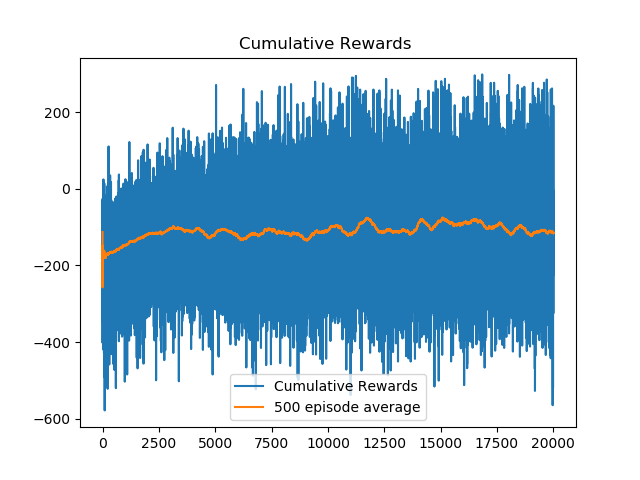
\includegraphics[width=\textwidth]{Lunar_rewards.png}
    \caption{Training performance of cumulative reward for Lunar Lander}
    \label{fig-Lunar}
\end{figure}
This clearly shows that the model is unable to learn anything as it is unable to get above 0 in average. It seems to land very rarely while testing. It seems to be able to navigate in the environment properly but is unable to achieve the goal of landing.
\section*{Question 3.2}
The lunar lander environment is more complex than the cartpole especially due to a couple of reasons.The sheer size of the discretized state space might mean that more exploration might be necessary for the model to learn a better policy that would help it land. Hence the discrete state space that ranges in the millions might be unable to converge effectively in any time frame. This might be strategies like not doing anything when it's above the landing site and then firing the thrusters really fast to land softly. The rewards structure for the lunar lander is also more delayed as landing is the last time step in an episode and that garners the most positive reward and also most of the time, firing the main thrusters the model accrues more negative rewards, hence the action space is filled with most actions that lead to negative rewards. This might just mean that the environment might need to train for much longer for the rewards from successfully landing to also update the state action values which are more in the beginning of the episode.  
\end{document}